
%%--------------------------------------------------
%% Serway: Physics for Scientists and Engineers
%%--------------------------------------------------


%% Chapter 03: Vectors
%%--------------------------------------------------


%% Table of Contents
%%--------------------------------------------------

%% 3.1 Coordinate Systems
%% 3.2 Vector and Scalar Quantities
%% 3.3 Some Properties of Vectors
%% 3.4 Components of a Vector and Unit Vectors


%% Serway Multiple Choice Questions
%%--------------------------------------------------

%% NOTE: On occasion, the notation A = [A, θ ] will be a shorthand notation for A = Acos θ ˆ i + Asin θ ˆ j .

\element{serway-mc}{
\begin{question}{serway-ch03-q01}
    If $\vec{\mathbf{A}} = [15, \ang{80}]$ and $\vec{\mathbf{B}} = 12\hat{\imath} - 16\hat{\jmath}$,
        what is the magnitude of $\vec{\mathbf{A}} - \vec{\mathbf{B}}$?
    \begin{multicols}{3}
    \begin{choices}
        \wrongchoice{\num{15}}
        \wrongchoice{\num{35}}
      \correctchoice{\num{32}}
        \wrongchoice{\num{5.0}}
        \wrongchoice{\num{23}}
    \end{choices}
    \end{multicols}
\end{question}
}

\element{serway-mc}{
\begin{question}{serway-ch03-q02}
    Vectors $\mathbf{A}$ and $\mathbf{B}$ are shown.
    \begin{center}
    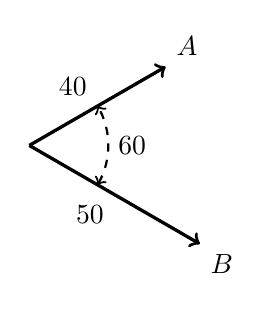
\begin{tikzpicture}[scale=0.5]
        \draw[very thick,->] (0,0) -- ++(+30:4)
            node[pos=1.0,anchor=south west] {$A$}
            node[pos=0.5,anchor=south east] {\num{40}};
        \draw[very thick,->] (0,0) -- ++(-30:5)
            node[pos=1.0,anchor=north west] {$B$}
            node[pos=0.5,anchor=north east] {\num{50}};
        \draw[thick,dashed,<->] (-30:2) arc (-30:30:2)
            node[pos=0.5,anchor=west] {\ang{60}};
    \end{tikzpicture}
    \end{center}
    What is the magnitude of a vector $\mathbf{C}$ if $\mathbf{C} = \mathbf{A} - \mathbf{B}$ ?
    \begin{multicols}{3}
    \begin{choices}
      \correctchoice{\num{46}}
        \wrongchoice{\num{10}}
        \wrongchoice{\num{30}}
        \wrongchoice{\num{78}}
        \wrongchoice{\num{90}}
    \end{choices}
    \end{multicols}
\end{question}
}

\element{serway-mc}{
\begin{question}{serway-ch03-q03}
    If $\mathbf{A} = 12\hat{\imath} - 16\hat{\jmath}$ and $\mathbf{B} = -24\hat{\imath} + 10\hat{\jmath}$,
        what is the magnitude of the vector $\mathbf{C} = 2 \mathbf{A} - \mathbf{B}$?
    \begin{multicols}{3}
    \begin{choices}
        \wrongchoice{\num{42}}
        \wrongchoice{\num{22}}
      \correctchoice{\num{64}}
        \wrongchoice{\num{90}}
        \wrongchoice{\num{13}}
    \end{choices}
    \end{multicols}
\end{question}
}

\element{serway-mc}{
\begin{question}{serway-ch03-q04}
    If $\vec{\mathbf{A}} = 12\hat{\imath} - 16\hat{\jmath}$ and $\vec{\mathbf{B}} = -24\hat{\imath} + 10\hat{\jmath}$,
        what is the direction of the vector $\vec{\mathbf{C}} = 2\vec{\mathbf{A}} - \vec{\mathbf{B}}$?
    \begin{multicols}{3}
    \begin{choices}
        \wrongchoice{\ang{-49}}
      \correctchoice{\ang{-41}}
        \wrongchoice{\ang{-90}}
        \wrongchoice{\ang{+49}}
        \wrongchoice{\ang{+21}}
    \end{choices}
    \end{multicols}
\end{question}
}

\element{serway-mc}{
\begin{question}{serway-ch03-q05}
    If $\vec{\mathbf{C}} = [\SI{10}{\meter}, \ang{30}]$ and $\vec{\mathbf{D}} = [\SI{25}{\meter}, \ang{130}]$,
        what is the magnitude of the sum of these two vectors?
    \begin{multicols}{3}
    \begin{choices}
        \wrongchoice{\SI{20}{\meter}}
        \wrongchoice{\SI{35}{\meter}}
        \wrongchoice{\SI{15}{\meter}}
      \correctchoice{\SI{25}{\meter}}
        \wrongchoice{\SI{50}{\meter}}
    \end{choices}
    \end{multicols}
\end{question}
}

\element{serway-mc}{
\begin{question}{serway-ch03-q06}
    If $\vec{\mathbf{C}} = [\SI{10}{\meter}, \ang{30}]$ and $\vec{\mathbf{D}} = [\SI{25}{\meter}, \ang{130}]$,
        what is the direction of the sum of these two vectors?
    \begin{multicols}{3}
    \begin{choices}
        \wrongchoice{\ang{17}}
        \wrongchoice{\ang{73}}
      \correctchoice{\ang{107}}
        \wrongchoice{\ang{163}}
        \wrongchoice{\ang{100}}
    \end{choices}
    \end{multicols}
\end{question}
}

\element{serway-mc}{
\begin{question}{serway-ch03-q07}
    A vector, $\vec{\mathbf{B}}$,
    when added to the vector $\vec{\mathbf{C}} = 3\hat{\imath} + 4\hat{\jmath}$ yields a resultant vector which is in the positive y direction and has a magnitude equal to that of $\vec{\mathbf{C}}$.
    What is the magnitude of $\vec{\mathbf{B}}$?
    \begin{multicols}{3}
    \begin{choices}
      \correctchoice{\num{3.2}}
        \wrongchoice{\num{6.3}}
        \wrongchoice{\num{9.5}}
        \wrongchoice{\num{18}}
        \wrongchoice{\num{5}}
    \end{choices}
    \end{multicols}
\end{question}
}

\element{serway-mc}{
\begin{question}{serway-ch03-q08}
    If vector $\vec{\mathbf{B}}$ is added to vector $\vec{\mathbf{A}}$,
        the result is $6\hat{\imath} + \hat{\jmath}$.
    If $\vec{\mathbf{B}}$ is subtracted from $\vec{\mathbf{A}}$,
        the result is $- 4\hat{\imath} + 7\hat{\jmath}$.
    What is the magnitude of $\vec{\mathbf{A}}$?
    \begin{multicols}{3}
    \begin{choices}
        \wrongchoice{\num{5.1}}
      \correctchoice{\num{4.1}}
        \wrongchoice{\num{5.4}}
        \wrongchoice{\num{5.8}}
        \wrongchoice{\num{8.2}}
    \end{choices}
    \end{multicols}
\end{question}
}

\element{serway-mc}{
\begin{question}{serway-ch03-q09}
    If $\vec{\mathbf{C}} = [\SI{2.5}{\centi\meter}, \ang{80}]$,
        i.e., the magnitude and direction of $\vec{\mathbf{C}}$ are \SI{2.5}{\centi\meter} and \ang{80},
    $\vec{\mathbf{D}} = [\SI{3.5}{\centi\meter}, \ang{120}]$,
        and $\vec{\mathbf{E}} = \vec{\mathbf{D}} - 2\vec{\mathbf{C}}$,
        what is the direction of $\vec{\mathbf{E}}$ (to the nearest degree)?
    \begin{multicols}{3}
    \begin{choices}
        \wrongchoice{\ang{247}}
        \wrongchoice{\ang{235}}
        \wrongchoice{\ang{243}}
      \correctchoice{\ang{216}}
        \wrongchoice{\ang{144}}
    \end{choices}
    \end{multicols}
\end{question}
}

\element{serway-mc}{
\begin{question}{serway-ch03-q10}
    If vector $\vec{\mathbf{C}}$ is added to vector $\vec{\mathbf{B}}$,
        the result is $- 9\hat{\imath} - 8\hat{\jmath}$.
    If $\vec{\mathbf{B}}$ is subtracted from $\vec{\mathbf{C}}$,
    the result is $5\hat{\imath} + 4\hat{\jmath}$.
        What is the direction of $\vec{\mathbf{B}}$ (to the nearest degree)?
    \begin{multicols}{3}
    \begin{choices}
        \wrongchoice{\ang{225}}
      \correctchoice{\ang{221}}
        \wrongchoice{\ang{230}}
        \wrongchoice{\ang{236}}
        \wrongchoice{\ang{206}}
    \end{choices}
    \end{multicols}
\end{question}
}

\element{serway-mc}{
\begin{question}{serway-ch03-q11}
    A vector $\vec{\mathbf{A}}$ is added to $\vec{\mathbf{B}} = 6\hat{\imath} - 8\hat{\jmath}$.
    The resultant vector is in the positive $x$ direction and has a magnitude equal to $\vec{\mathbf{A}}$.
    What is the magnitude of $\vec{\mathbf{A}}$?
    \begin{multicols}{3}
    \begin{choices}
        \wrongchoice{\num{11}}
        \wrongchoice{\num{5.1}}
        \wrongchoice{\num{7.1}}
      \correctchoice{\num{8.3}}
        \wrongchoice{\num{12.2}}
    \end{choices}
    \end{multicols}
\end{question}
}

\element{serway-mc}{
\begin{question}{serway-ch03-q12}
    A vector $\vec{\mathbf{A}}$ is added to $\vec{\mathbf{B}} = 6\hat{\imath} - 8\hat{\jmath}$.
    The resultant vector is in the positive $x$ direction and has a magnitude equal to that of $\vec{\mathbf{A}}$.
    What is the direction of $\vec{\mathbf{A}}$?
    \begin{multicols}{3}
    \begin{choices}
      \correctchoice{\ang{74}}
        \wrongchoice{\ang{100}}
        \wrongchoice{\ang{-81}}
        \wrongchoice{\ang{-62}}
        \wrongchoice{\ang{106}}
    \end{choices}
    \end{multicols}
\end{question}
}

\element{serway-mc}{
\begin{question}{serway-ch03-q13}
    %If two collinear vectors $\vec{\mathbf{A}}$ and $\vec{\mathbf{B}}$ are added,
    %    the resultant has a magnitude equal to \num{4.0}.
    %If $\vec{\mathbf{B}}$ is subtracted from $\vec{\mathbf{A}}$,
    %    the resultant has a magnitude equal to \num{8.0}.
    %What is the magnitude of $\vec{\mathbf{B}}$?
    %% NOTE: removed the term magnitude
    If two collinear vectors $\vec{\mathbf{A}}$ and $\vec{\mathbf{B}}$ are added,
        the resultant is equal to \num{4.0}.
    If $\vec{\mathbf{B}}$ is subtracted from $\vec{\mathbf{A}}$,
        the resultant is equal to \num{8.0}.
    What is the magnitude of $\vec{\mathbf{B}}$?
    \begin{multicols}{3}
    \begin{choices}
      \correctchoice{\num{2.0}}
        \wrongchoice{\num{3.0}}
        \wrongchoice{\num{4.0}}
        \wrongchoice{\num{5.0}}
        \wrongchoice{\num{6.0}}
    \end{choices}
    \end{multicols}
\end{question}
}

\element{serway-mc}{
\begin{question}{serway-ch03-q14}
    %% NOTE: removed the term magnitude
    If two collinear vectors $\vec{\mathbf{A}}$ and $\vec{\mathbf{B}}$ are added,
        the resultant is equal to \num{4.0}.
    If $\vec{\mathbf{B}}$ is subtracted from $\vec{\mathbf{A}}$,
        the resultant is equal to \num{8.0}.
    What is the magnitude of $\vec{\mathbf{A}}$?
    \begin{multicols}{3}
    \begin{choices}
        \wrongchoice{\num{2.0}}
        \wrongchoice{\num{3.0}}
        \wrongchoice{\num{4.0}}
        \wrongchoice{\num{5.0}}
      \correctchoice{\num{6.0}}
    \end{choices}
    \end{multicols}
\end{question}
}

\element{serway-mc}{
\begin{question}{serway-ch03-q15}
    When vector $\vec{\mathbf{A}}$ is added to vector $\vec{\mathbf{B}}$,
        which has a magnitude of \num{5.0},
        the vector representing their sum is perpendicular to $\vec{\mathbf{A}}$ and has a magnitude that is twice that of $\vec{\mathbf{A}}$.
    What is the magnitude of $\vec{\mathbf{A}}$?
    \begin{multicols}{3}
    \begin{choices}
      \correctchoice{\num{2.2}}
        \wrongchoice{\num{2.5}}
        \wrongchoice{\num{4.5}}
        \wrongchoice{\num{5.0}}
        \wrongchoice{\num{7.0}}
    \end{choices}
    \end{multicols}
\end{question}
}

\element{serway-mc}{
\begin{question}{serway-ch03-q16}
    Starting from one oasis, a camel walks \SI{25}{\kilo\meter} in a direction \ang{30} south of west and then walks \SI{30}{\kilo\meter} toward the north to a second oasis.
    What distance separates the two oases?
    \begin{multicols}{3}
    \begin{choices}
        \wrongchoice{\SI{15}{\kilo\meter}}
        \wrongchoice{\SI{48}{\kilo\meter}}
      \correctchoice{\SI{28}{\kilo\meter}}
        \wrongchoice{\SI{53}{\kilo\meter}}
        \wrongchoice{\SI{55}{\kilo\meter}}
    \end{choices}
    \end{multicols}
\end{question}
}

\element{serway-mc}{
\begin{question}{serway-ch03-q17}
    Starting from one oasis,
    a camel walks \SI{25}{\kilo\meter} in a direction \ang{30} south of west and then walks \SI{30}{\kilo\meter} toward the north to a second oasis.
    What is the direction from the first oasis to the second oasis?
    \begin{multicols}{2}
    \begin{choices}
        \wrongchoice{\ang{21} N of W}
        \wrongchoice{\ang{39} W of N}
        \wrongchoice{\ang{69} N of W}
      \correctchoice{\ang{51} W of N}
        \wrongchoice{\ang{42} W of N}
    \end{choices}
    \end{multicols}
\end{question}
}

\newcommand{\serwayChThreeQEighteen}{
\begin{tikzpicture}[scale=0.8,font=\small]
    %% Draw X Y axes
    \draw[->] (0,-3) -- (0,+3)
        node[pos=1.0,anchor=south] {$y$};
    \draw[->] (-3,0) -- (+3,0)
        node[pos=1.0,anchor=west] {$x$};
    %% Draw vectors
    \draw[very thick,->] (0,0) -- ++(30:4.33)
        node[anchor=south west] {\SI{65.0}{\newton}};
    \draw[very thick,->] (0,0) -- ++(180:2)
        node[anchor=south west] {\SI{30.0}{\newton}};
    \draw[very thick,->] (0,0) -- ++(250:1.33)
        node[anchor=north east] {\SI{20.0}{\newton}};
    %% Angles
    \draw[->] (1,0) arc (0:30:1)
        node[pos=0.5,anchor=west] {\ang{30}};
    \draw[->] (230:1) arc (230:250:1);
    \draw[->] (290:1) arc (290:270:1)
        node[pos=0,anchor=west] {\ang{20}};
\end{tikzpicture}
}

\element{serway-mc}{
\begin{question}{serway-ch03-q18}
    The three forces shown act on a particle.
    \begin{center}
        \serwayChThreeQEighteen
    \end{center}
    What is the magnitude of the resultant of these three forces?
    \begin{multicols}{3}
    \begin{choices}
        \wrongchoice{\SI{27.0}{\newton}}
        \wrongchoice{\SI{33.2}{\newton}}
        \wrongchoice{\SI{36.3}{\newton}}
      \correctchoice{\SI{23.8}{\newton}}
        \wrongchoice{\SI{105}{\newton}}
    \end{choices}
    \end{multicols}
\end{question}
}

\element{serway-mc}{
\begin{question}{serway-ch03-q19}
    The three forces shown act on a particle.
    \begin{center}
        \serwayChThreeQEighteen
    \end{center}
    What is the direction of the resultant of these three forces,
    %% changed wording to make clear
        with respect to the $y$-axis?
    \begin{multicols}{3}
    \begin{choices}
      \correctchoice{\ang{35}}
        \wrongchoice{\ang{45}}
        \wrongchoice{\ang{65}}
        \wrongchoice{\ang{55}}
        \wrongchoice{\ang{85}}
    \end{choices}
    \end{multicols}
\end{question}
}

\element{serway-mc}{
\begin{question}{serway-ch03-q20}
    If vector $\vec{\mathbf{C}}$ is added to vector $\vec{\mathbf{D}}$,
    the result is a third vector that is perpendicular to $\vec{\mathbf{D}}$ and has a magnitude equal to $3\vec{\mathbf{D}}$.
    What is the ratio of the magnitude of $\vec{\mathbf{C}}$ to that of $\vec{\mathbf{D}}$?
    \begin{multicols}{3}
    \begin{choices}
        \wrongchoice{\num{1.8}}
        \wrongchoice{\num{2.2}}
      \correctchoice{\num{3.2}}
        \wrongchoice{\num{1.3}}
        \wrongchoice{\num{1.6}}
    \end{choices}
    \end{multicols}
\end{question}
}

%\element{serway-mc}{
%\begin{question}{serway-ch03-q21}
%    A child starts at one corner of a cubical jungle gym in a playground and climbs up to the diagonally opposite corner.
%    \begin{center}
%    \begin{tikzpicture}
%        %% NOTE: TODO: draw tikz \foreach
%    \end{tikzpicture}
%    \end{center}
%    The original corner is the coordinate origin,
%        and the $x$-, $y$- and $z$-axes are oriented along the jungle gym edges.
%    The length of each side is \SI{2}{\meter}.
%    The child's displacement is:
%    \begin{multicols}{2}
%    \begin{choices}
%      \correctchoice{$2\hat{\imath}   + 2\hat{\jmath}   + 2\hat{k}$}
%        \wrongchoice{$2.8\hat{\imath} + 2\hat{\jmath}   + 2\hat{k}$}
%        \wrongchoice{$2\hat{\imath}   + 2\hat{\jmath}   + 2.8\hat{k}$}
%        \wrongchoice{$2\hat{\imath}   + 2\hat{\jmath}   + 3.5\hat{k}$}
%        \wrongchoice{$3.5\hat{\imath} + 3.5\hat{\jmath} + 3.5\hat{k}$}
%    \end{choices}
%    \end{multicols}
%\end{question}
%}

\element{serway-mc}{
\begin{question}{serway-ch03-q22}
    The displacement of the tip of the \SI{10}{\centi\meter} long minute hand of a clock between 12:15 A.M. and 12:45 P.M. is:
    \begin{multicols}{2}
    \begin{choices}
        \wrongchoice{\SI{10}{\centi\meter}, \ang{90}}
        \wrongchoice{\SI{10}{\centi\meter}, \ang{180}}
        \wrongchoice{\SI{10}{\centi\meter}, \ang{4500}}
      \correctchoice{\SI{20}{\centi\meter}, \ang{180}}
        \wrongchoice{\SI{20}{\centi\meter}, \ang{540}}
    \end{choices}
    \end{multicols}
\end{question}
}

\element{serway-mc}{
\begin{question}{serway-ch03-q23}
    A student decides to spend spring break by driving 50 miles due east,
        then 50 miles \num{30} degrees south of east,
        then 50 miles \num{30} degrees south of that direction,
        and to continue to drive 50 miles deviating by \num{30} degrees each time until he returns to his original position.
    How far will he drive, and how many vectors must he sum to calculate his displacement?
    \begin{multicols}{2}
    \begin{choices}
        \wrongchoice{\SI{0}{\mile}, \num{0}}
        \wrongchoice{\SI{0}{\mile}, \num{8}}
        \wrongchoice{\SI{0}{\mile}, \num{12}}
        \wrongchoice{\SI{400}{\mile}, \num{8}}
      \correctchoice{\SI{600}{\mile}, \num{12}}
    \end{choices}
    \end{multicols}
\end{question}
}

\element{serway-mc}{
\begin{question}{serway-ch03-q24}
    Jane plans to fly from Binghampton, New York, to Springfield, Massachusetts,
        about \SI{280}{\kilo\meter} due east of Binghampton.
    She heads due east at \SI{280}{\kilo\meter\per\hour} for one hour but finds herself at Keene,
        which is \SI{294}{\kilo\meter} from Binghampton in a direction \num{17.8} degrees north of due east.
    What was the wind velocity?
    \begin{multicols}{2}
    \begin{choices}
        \wrongchoice{\SI{14}{\kilo\meter\per\hour}, E}
        \wrongchoice{\SI{14}{\kilo\meter\per\hour}, W}
        \wrongchoice{\SI{14}{\kilo\meter\per\hour}, N}
        \wrongchoice{\SI{90}{\kilo\meter\per\hour}, S}
      \correctchoice{\SI{90}{\kilo\meter\per\hour}, N}
    \end{choices}
    \end{multicols}
\end{question}
}

\element{serway-mc}{
\begin{question}{serway-ch03-q25}
    Given that $\vec{\mathbf{A}} + 2\vec{\mathbf{B}} = x_1\hat{\imath} + y_1\hat{\jmath}$ and $2\vec{\mathbf{A}} - \vec{\mathbf{B}} = x_2\hat{\imath} + y_2\hat{\jmath}$,
        what is $\vec{\mathbf{A}}$?
    \begin{choices}
      \correctchoice{$\vec{\mathbf{A}} = \dfrac{1}{5} \left(x_1+2x_2\right)\hat{\imath} + \dfrac{1}{5}\left(y_1+2y_2\right)\hat{\jmath}$}
        \wrongchoice{$\vec{\mathbf{A}} = \dfrac{1}{5} \left(x_1-2x_2\right)\hat{\imath} + \dfrac{1}{5}\left(y_1-2y_2\right)\hat{\jmath}$}
        \wrongchoice{$\vec{\mathbf{A}} = \dfrac{1}{5} \left(x_1+4x_2\right)\hat{\imath} + \dfrac{1}{5}\left(y_1+2y_2\right)\hat{\jmath}$}
        \wrongchoice{$\vec{\mathbf{A}} = \dfrac{1}{5} \left(x_1+4x_2\right)\hat{\imath} + \dfrac{1}{5}\left(y_1+4y_2\right)\hat{\jmath}$}
        \wrongchoice{$\vec{\mathbf{A}} = \dfrac{1}{5} \left(x_1+4x_2\right)\hat{\imath} + \dfrac{1}{5}\left(y_1-4y_2\right)\hat{\jmath}$}
    \end{choices}
\end{question}
}

\element{serway-mc}{
\begin{question}{serway-ch03-q26}
    Given that $\vec{\mathbf{A}} + \vec{\mathbf{B}} = x_1\hat{\imath} + y_1\hat{\jmath}$ and $\vec{\mathbf{A}} - \vec{\mathbf{B}} = x_2\hat{\imath} + y_2\hat{\jmath}$,
        what is $\vec{\mathbf{A}}$?
    \begin{choices}
        \wrongchoice{$\vec{\mathbf{A}} = \dfrac{1}{2} \left(x_1-x_2\right)\hat{\imath} + \dfrac{1}{2}\left(y_1-y_2\right)\hat{\jmath}$}
        \wrongchoice{$\vec{\mathbf{A}} = \dfrac{1}{2} \left(x_1+x_2\right)\hat{\imath} + \dfrac{1}{2}\left(y_1-y_2\right)\hat{\jmath}$}
        \wrongchoice{$\vec{\mathbf{A}} = \dfrac{1}{2} \left(x_1-x_2\right)\hat{\imath} + \dfrac{1}{2}\left(y_1+y_2\right)\hat{\jmath}$}
      \correctchoice{$\vec{\mathbf{A}} = \dfrac{1}{2} \left(x_1+x_2\right)\hat{\imath} + \dfrac{1}{2}\left(y_1+y_2\right)\hat{\jmath}$}
        \wrongchoice{$\vec{\mathbf{A}} = \dfrac{1}{2} \left(x_1+x_2\right)\hat{\imath}$}
    \end{choices}
\end{question}
}

\element{serway-mc}{
\begin{question}{serway-ch03-q27}
    Given that $\vec{\mathbf{A}} + \vec{\mathbf{B}} = x_1\hat{\imath} + y_1\hat{\jmath}$ and $\vec{\mathbf{A}} - \vec{\mathbf{B}} = x_2\hat{\imath} + y_2\hat{\jmath}$,
        what is $\vec{\mathbf{B}}$?
    \begin{choices}
      \correctchoice{$\vec{\mathbf{B}} = \dfrac{1}{2} \left(x_1-x_2\right)\hat{\imath} + \dfrac{1}{2}\left(y_1-y_2\right)\hat{\jmath}$}
        \wrongchoice{$\vec{\mathbf{B}} = \dfrac{1}{2} \left(x_1+x_2\right)\hat{\imath} + \dfrac{1}{2}\left(y_1-y_2\right)\hat{\jmath}$}
        \wrongchoice{$\vec{\mathbf{B}} = \dfrac{1}{2} \left(x_1-x_2\right)\hat{\imath} + \dfrac{1}{2}\left(y_1+y_2\right)\hat{\jmath}$}
        \wrongchoice{$\vec{\mathbf{B}} = \dfrac{1}{2} \left(x_1+x_2\right)\hat{\imath} + \dfrac{1}{2}\left(y_1+y_2\right)\hat{\jmath}$}
        \wrongchoice{$\vec{\mathbf{B}} = \dfrac{1}{2} \left(x_1+x_2\right)\hat{\jmath}$}
    \end{choices}
\end{question}
}

\element{serway-mc}{
\begin{question}{serway-ch03-q28}
    The diagram below shows 3 vectors which sum to zero, all of equal length.
    \begin{center}
    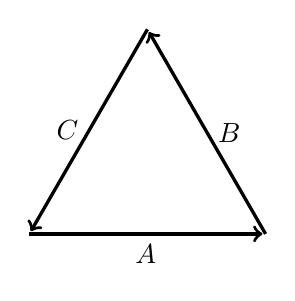
\begin{tikzpicture}
        \draw[very thick,->] (0,0) -- ++ (0:2.96) node[pos=0.5,anchor=north] {$A$};
        \draw[very thick,->] (60:3) -- ++ (240:2.96) node[pos=0.5,anchor=east] {$C$};
        \draw[very thick,->] (3,0) -- ++ (120:2.96) node[pos=0.5,anchor=west] {$B$};
    \end{tikzpicture}
    \end{center}
    Which statement below is true?
    \begin{multicols}{2}
    \begin{choices}
        \wrongchoice{$\vec{\mathbf{A}} + \vec{\mathbf{B}} = \vec{\mathbf{A}} - \vec{\mathbf{C}}$}
        \wrongchoice{$\vec{\mathbf{A}} + \vec{\mathbf{B}} = \vec{\mathbf{B}} - \vec{\mathbf{C}}$}
        \wrongchoice{$\vec{\mathbf{A}} - \vec{\mathbf{B}} = 2\vec{\mathbf{A}} - \vec{\mathbf{C}}$}
      \correctchoice{$\vec{\mathbf{A}} - \vec{\mathbf{B}} = 2\vec{\mathbf{A}} + \vec{\mathbf{C}}$}
        \wrongchoice{$2\vec{\mathbf{A}} + 2\vec{\mathbf{B}} = 2\vec{\mathbf{C}}$}
        %% do not add a sixth option for symmetry
        %% since each individually must be compared
    \end{choices}
    \end{multicols}
\end{question}
}

\element{serway-mc}{
\begin{questionmult}{serway-ch03-q29}
    Which statement is true about the unit vectors $\hat{\imath}$,
        $\hat{\jmath}$ and $\hat{k}$?
    \begin{choices}
        \wrongchoice{Their directions are defined by a left-handed coordinate system.}
      \correctchoice{The angle between any two is \num{90} degrees.}
        \wrongchoice{Each has a length of \SI{1}{\meter}.}
        \wrongchoice{If $\hat{\imath}$ is directed east and $\hat{\jmath}$ is directed south, $\hat{k}$ points up out of the surface.}
        %\wrongchoice{All of the provided options.}
    \end{choices}
\end{questionmult}
}

\element{serway-mc}{
\begin{question}{serway-ch03-q30}
    Vectors $\vec{\mathbf{A}}$ and $\vec{\mathbf{B}}$ have equal magnitudes.
    Which statement is always true?
    \begin{choices}
        \wrongchoice{$\vec{\mathbf{A}} + \vec{\mathbf{B}} = 0$.}
        \wrongchoice{$\vec{\mathbf{A}} - \vec{\mathbf{B}} = 0$.}
      \correctchoice{$\vec{\mathbf{A}} - \vec{\mathbf{B}}$ is perpendicular to $\vec{\mathbf{A}} + \vec{\mathbf{B}}$.}
        \wrongchoice{$\vec{\mathbf{B}} - \vec{\mathbf{A}}$ is perpendicular to $\vec{\mathbf{A}} - \vec{\mathbf{B}}$.}
        \wrongchoice{The magnitude of $\vec{\mathbf{A}} - \vec{\mathbf{B}}$ equals the magnitude of $\vec{\mathbf{A}} + \vec{\mathbf{B}}$.}
    \end{choices}
\end{question}
}

\element{serway-mc}{
\begin{question}{serway-ch03-q31}
    When three vectors, $\vec{\mathbf{A}}$ , $\vec{\mathbf{B}}$,
        and $\vec{\mathbf{C}}$ are placed head to tail,
        the vector sum $\vec{\mathbf{A}} + \vec{\mathbf{B}} + \vec{\mathbf{C}} = 0$.
    If the vectors all have the same magnitude,
        the angle between the directions of any two adjacent vectors is:
    \begin{multicols}{3}
    \begin{choices}
        \wrongchoice{\ang{30}}
        \wrongchoice{\ang{60}}
        \wrongchoice{\ang{90}}
      \correctchoice{\ang{120}}
        \wrongchoice{\ang{150}}
    \end{choices}
    \end{multicols}
\end{question}
}

\newcommand{\serwayChThreeQThirtyTwo}{
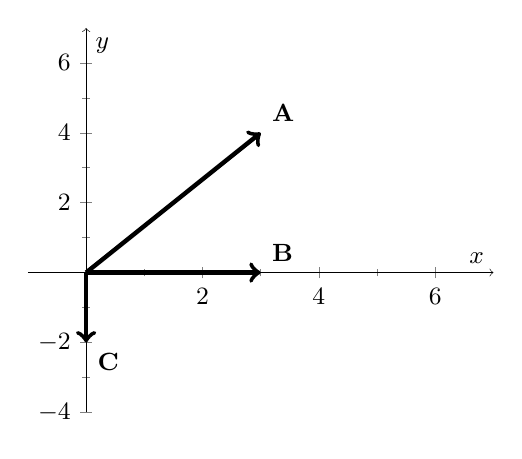
\begin{tikzpicture}[font=\small]
    \begin{axis}[
        clip=false,
        axis y line=middle,
        axis x line=middle,
        axis line style={->},
        xlabel={$x$},
        xtick={0,2,4,6},
        minor x tick num=1,
        ylabel={$y$},
        ytick={-4,-2,0,2,4,6},
        minor y tick num=1,
        %grid=major,
        xmin=-1,xmax=7,
        ymin=-4,ymax=7,
        width=0.618\columnwidth,
        very thin,
    ]
    \draw[ultra thick,->] (axis cs:0,0) -- (axis cs:3,4) node[anchor=south west] {$\mathbf{A}$};
    \draw[ultra thick,->] (axis cs:0,0) -- (axis cs:3,0) node[anchor=south west] {$\mathbf{B}$};
    \draw[ultra thick,->] (axis cs:0,0) -- (axis cs:0,-2) node[anchor=north west] {$\mathbf{C}$};
    \end{axis}
\end{tikzpicture}
}

\element{serway-mc}{
\begin{question}{serway-ch03-q32}
    The vectors $\vec{\mathbf{A}}$, $\vec{\mathbf{B}}$, and $\vec{\mathbf{C}}$ are shown below.
    \begin{center}
        \serwayChThreeQThirtyTwo
    \end{center}
    Which diagram below correctly represents $\vec{\mathbf{A}} + \vec{\mathbf{B}} + \vec{\mathbf{C}}$?
    \begin{multicols}{2}
    \begin{choices}
        \AMCboxDimensions{down=-2.0em}
        \wrongchoice{
            \begin{tikzpicture}[font=\small]
                \begin{axis}[
                    clip=false,
                    axis y line=middle,
                    axis x line=middle,
                    axis line style={->},
                    xlabel={$x$},
                    xtick={0,2,4,6},
                    xticklabels={},
                    minor x tick num=1,
                    ylabel={$y$},
                    ytick={-8,-6,-4,-2,0,2,4,6,8},
                    yticklabels={},
                    minor y tick num=1,
                    xmin=-1,xmax=7,
                    ymin=-4,ymax=7,
                    width=1.00\columnwidth,
                ]
                \draw[ultra thick,->] (axis cs:0,0) -- (axis cs:6,4);
                \end{axis}
            \end{tikzpicture}
        }
        %% NOTE: ans is b
        \correctchoice{
            \begin{tikzpicture}[font=\small]
                \begin{axis}[
                    clip=false,
                    axis y line=middle,
                    axis x line=middle,
                    axis line style={->},
                    xlabel={$x$},
                    xtick={0,2,4,6},
                    xticklabels={},
                    minor x tick num=1,
                    ylabel={$y$},
                    ytick={-8,-6,-4,-2,0,2,4,6,8},
                    yticklabels={},
                    minor y tick num=1,
                    xmin=-1,xmax=7,
                    ymin=-4,ymax=7,
                    width=1.00\columnwidth,
                ]
                \draw[ultra thick,->] (axis cs:0,0) -- (axis cs:6,2);
                \end{axis}
            \end{tikzpicture}
        }
        \wrongchoice{
            \begin{tikzpicture}[font=\small]
                \begin{axis}[
                    clip=false,
                    axis y line=middle,
                    axis x line=middle,
                    axis line style={->},
                    xlabel={$x$},
                    xtick={0,2,4,6},
                    xticklabels={},
                    minor x tick num=1,
                    ylabel={$y$},
                    ytick={-8,-6,-4,-2,0,2,4,6,8},
                    yticklabels={},
                    minor y tick num=1,
                    xmin=-1,xmax=7,
                    ymin=-4,ymax=7,
                    width=1.00\columnwidth,
                ]
                \draw[ultra thick,->] (axis cs:0,0) -- (axis cs:6,-2);
                \end{axis}
            \end{tikzpicture}
        }
        \wrongchoice{
            \begin{tikzpicture}[font=\small]
                \begin{axis}[
                    clip=false,
                    axis y line=middle,
                    axis x line=middle,
                    axis line style={->},
                    xlabel={$x$},
                    xtick={0,2,4,6},
                    xticklabels={},
                    minor x tick num=1,
                    ylabel={$y$},
                    ytick={-8,-6,-4,-2,0,2,4,6,8},
                    yticklabels={},
                    minor y tick num=1,
                    xmin=-1,xmax=7,
                    ymin=-4,ymax=7,
                    width=1.00\columnwidth,
                ]
                \draw[ultra thick,->] (axis cs:0,0) -- (axis cs:6,-4);
                \end{axis}
            \end{tikzpicture}
        }
        \wrongchoice{
            \begin{tikzpicture}[font=\small]
                \begin{axis}[
                    clip=false,
                    axis y line=middle,
                    axis x line=middle,
                    axis line style={->},
                    xlabel={$x$},
                    xtick={0,2,4,6},
                    xticklabels={},
                    minor x tick num=1,
                    ylabel={$y$},
                    ytick={-8,-6,-4,-2,0,2,4,6,8},
                    yticklabels={},
                    minor y tick num=1,
                    xmin=-1,xmax=7,
                    ymin=-4,ymax=7,
                    width=1.00\columnwidth,
                ]
                \draw[ultra thick,->] (axis cs:0,0) -- (axis cs:6,0);
                \end{axis}
            \end{tikzpicture}
        }
    \end{choices}
    \end{multicols}
\end{question}
}

\element{serway-mc}{
\begin{question}{serway-ch03-q33}
    The vectors $\vec{\mathbf{A}}$, $\vec{\mathbf{B}}$, and $\vec{\mathbf{C}}$ are shown below.
    \begin{center}
        \serwayChThreeQThirtyTwo
    \end{center}
    Which diagram below correctly represents $\vec{\mathbf{A}} - \vec{\mathbf{B}} + 2\vec{\mathbf{C}}$?
    \begin{multicols}{2}
    \begin{choices}
        \AMCboxDimensions{down=-2.5em}
        %% NOTE: ans is a
        \correctchoice{
            \begin{tikzpicture}[font=\small]
                \begin{axis}[
                    clip=false,
                    axis y line=middle,
                    axis x line=middle,
                    axis line style={->},
                    xlabel={$x$},
                    xtick={0,2,4,6},
                    xticklabels={},
                    minor x tick num=1,
                    ylabel={$y$},
                    ytick={-8,-6,-4,-2,0,2,4,6,8},
                    yticklabels={},
                    minor y tick num=1,
                    xmin=-1,xmax=7,
                    ymin=-8,ymax=8,
                    width=1.00\columnwidth,
                ]
                \draw[fill] (axis cs:0,0) circle (2pt);
                \end{axis}
            \end{tikzpicture}
        }
        \wrongchoice{
            \begin{tikzpicture}[font=\small]
                \begin{axis}[
                    clip=false,
                    axis y line=middle,
                    axis x line=middle,
                    axis line style={->},
                    xlabel={$x$},
                    xtick={0,2,4,6},
                    xticklabels={},
                    minor x tick num=1,
                    ylabel={$y$},
                    ytick={-8,-6,-4,-2,0,2,4,6,8},
                    yticklabels={},
                    minor y tick num=1,
                    xmin=-1,xmax=7,
                    ymin=-8,ymax=8,
                    width=1.00\columnwidth,
                ]
                \draw[ultra thick,->] (axis cs:0,0) -- (axis cs:0,-2);
                \end{axis}
            \end{tikzpicture}
        }
        \wrongchoice{
            \begin{tikzpicture}[font=\small]
                \begin{axis}[
                    clip=false,
                    axis y line=middle,
                    axis x line=middle,
                    axis line style={->},
                    xlabel={$x$},
                    xtick={0,2,4,6},
                    xticklabels={},
                    xticklabels={},
                    minor x tick num=1,
                    ylabel={$y$},
                    ytick={-8,-6,-4,-2,0,2,4,6,8},
                    yticklabels={},
                    minor y tick num=1,
                    xmin=-1,xmax=7,
                    ymin=-8,ymax=8,
                    width=1.00\columnwidth,
                ]
                \draw[ultra thick,->] (axis cs:0,0) -- (axis cs:0,+2);
                \end{axis}
            \end{tikzpicture}
        }
        \wrongchoice{
            \begin{tikzpicture}[font=\small]
                \begin{axis}[
                    clip=false,
                    axis y line=middle,
                    axis x line=middle,
                    axis line style={->},
                    xlabel={$x$},
                    xtick={0,2,4,6},
                    xticklabels={},
                    minor x tick num=1,
                    ylabel={$y$},
                    ytick={-8,-6,-4,-2,0,2,4,6,8},
                    yticklabels={},
                    minor y tick num=1,
                    xmin=-1,xmax=7,
                    ymin=-8,ymax=8,
                    width=1.00\columnwidth,
                ]
                \draw[ultra thick,->] (axis cs:0,0) -- (axis cs:0,-8);
                \end{axis}
            \end{tikzpicture}
        }
        \wrongchoice{
            \begin{tikzpicture}[font=\small]
                \begin{axis}[
                    clip=false,
                    axis y line=middle,
                    axis x line=middle,
                    axis line style={->},
                    xlabel={$x$},
                    xtick={0,2,4,6},
                    xticklabels={},
                    minor x tick num=1,
                    ylabel={$y$},
                    ytick={-8,-6,-4,-2,0,2,4,6,8},
                    yticklabels={},
                    minor y tick num=1,
                    xmin=-1,xmax=7,
                    ymin=-8,ymax=8,
                    width=1.00\columnwidth,
                ]
                \draw[ultra thick,->] (axis cs:0,0) -- (axis cs:0,8);
                \end{axis}
            \end{tikzpicture}
        }
    \end{choices}
    \end{multicols}
\end{question}
}

\newcommand{\serwayChThreeQThirtyFour}{
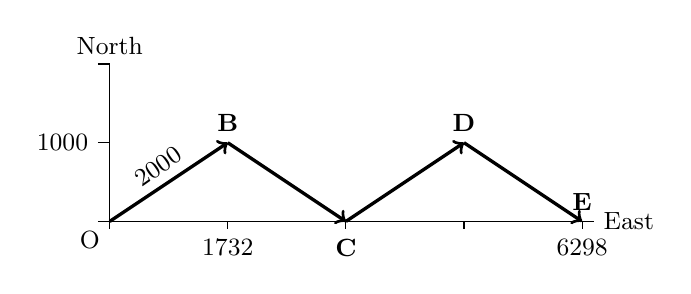
\begin{tikzpicture}[xscale=1.5,font=\small]
    %% E--W and S--N
    \draw (0,0) -- (4.1,0) node[anchor=west] {East};
    \draw (0,0) -- (0,2) node[anchor=south] {North};
    %% NOTE: letter O for origin
    \node[anchor=north east] at (0,0)  {O};
    %% x-axis ticks
    \foreach \x in {0,1,2,3,4}
        \draw (\x,0) -- (\x,-0.1);
    \node[anchor=north] at (1,-0.1) {\SI{1732}{\meter}};
    \node[anchor=north] at (2,-0.1) {$\mathbf{C}$};
    \node[anchor=north] at (4,-0.1) {\SI{6298}{\meter}};
    %% y-axis ticks/lablels
    \foreach \y in {0,1,2}
        \draw (-0.1,\y) -- (0,\y);
    \node[anchor=east] at (-0.1,1) {\SI{1000}{\meter}};
    %% path vectors
    \draw[very thick,->] (0,0) -- (1,1)
        node[pos=0.5,anchor=south,rotate=35] {\SI{2000}{\meter}}
        node[pos=1.0,anchor=south] {$\mathbf{B}$};
    \draw[very thick,->] (1,1) -- (2,0);
    \draw[very thick,->] (2,0) -- (3,1) node[anchor=south] {$\mathbf{D}$};
    \draw[very thick,->] (3,1) -- (4,0) node[anchor=south] {$\mathbf{E}$};
\end{tikzpicture}
}

\element{serway-mc}{
\begin{question}{serway-ch03-q34}
    The diagram below shows the path taken by a sailboat tacking sideways
        because it cannot sail directly into the wind.
    \begin{center}
        \serwayChThreeQThirtyFour
    \end{center}
    The total distance it travels is:
    \begin{multicols}{3}
    \begin{choices}
        \wrongchoice{\SI{1000}{\meter}}
        \wrongchoice{\SI{1732}{\meter}}
        \wrongchoice{\SI{2000}{\meter}}
        \wrongchoice{\SI{6298}{\meter}}
      \correctchoice{\SI{8000}{\meter}}
    \end{choices}
    \end{multicols}
\end{question}
}

\element{serway-mc}{
\begin{question}{serway-ch03-q35}
    The diagram below shows the path taken by a sailboat tacking
        sideways because it cannot sail directly into the wind.
    \begin{center}
        \serwayChThreeQThirtyFour
    \end{center}
    The total displacement of the sailboat,
    the vector sum of its displacements $\mathbf{OB}$,
        $\mathbf{BC}$, $\mathbf{CD}$ and $\mathbf{DE}$, is
    \begin{multicols}{2}
    \begin{choices}
        \wrongchoice{\SI{1 732}{\meter}, East.}
        \wrongchoice{\SI{2 000}{\meter}, Northeast.}
      \correctchoice{\SI{6 298}{\meter}, East.}
        \wrongchoice{\SI{8 000}{\meter}, Southeast.}
        \wrongchoice{\SI{8 000}{\meter}, East.}
    \end{choices}
    \end{multicols}
\end{question}
}

\element{serway-mc}{
\begin{question}{serway-ch03-q36}
    Each of two vectors, $\vec{\mathbf{D}}_1$ and $\vec{\mathbf{D}}_2$,
        lies along a coordinate axis in the $x$-$y$ plane.
    Each vector has its tail at the origin,
        and the dot product of the two vectors is
        $\mathbf{D_1}\cdot\mathbf{D_2} = 0$.
    Which possibility is correct?
    \begin{choices}
        \wrongchoice{$\vec{\mathbf{D}}_1$ and $\vec{\mathbf{D}}_2$ both lie along the positive $x$-axis.}
        \wrongchoice{$\vec{\mathbf{D}}_1$ lies along the positive $x$-axis.  $\vec{\mathbf{D}}_2$ lies along the negative $x$-axis.}
        \wrongchoice{$\vec{\mathbf{D}}_1$ and $\vec{\mathbf{D}}_2$ both lie along the positive $y$-axis.}
      \correctchoice{$\vec{\mathbf{D}}_1$ lies along the negative $x$-axis.  $\vec{\mathbf{D}}_2$ lies along the negative $y$-axis.}
        \wrongchoice{$\vec{\mathbf{D}}_1$ lies along the positive $y$-axis.  $\vec{\mathbf{D}}_2$ lies along the negative $y$-axis.}
    \end{choices}
\end{question}
}

\element{serway-mc}{
\begin{question}{serway-ch03-q37}
    Each of two vectors, $\vec{\mathbf{D}}_1$ and $\vec{\mathbf{D}}_2$,
        lies along a coordinate axis in the $x$-$y$ plane.
    Each vector has its tail at the origin,
        and the dot product of the two vectors is
        $\mathbf{D_1}\cdot\mathbf{D_2} = -|\vec{\mathbf{D}}_1 |\vec{\mathbf{D}}_2|$.
    Which possibility is correct?
    \begin{choices}
        \wrongchoice{$\vec{\mathbf{D}}_1$ and $\vec{\mathbf{D}}_2$ both lie along the positive $x$-axis.}
      \correctchoice{$\vec{\mathbf{D}}_1$ lies along the positive $x$-axis. $\vec{\mathbf{D}}_2$ lies along the negative $x$-axis.}
        \wrongchoice{$\vec{\mathbf{D}}_1$ and $\vec{\mathbf{D}}_2$ both lie along the positive $y$-axis.}
        \wrongchoice{$\vec{\mathbf{D}}_1$ lies along the negative $x$-axis. $\vec{\mathbf{D}}_2$ lies along the negative $y$-axis.}
        %% NOTE: changed from
        %\wrongchoice{$\vec{\mathbf{D}}_1$ lies along the positive $y$-axis. $\vec{\mathbf{D}}_2$ lies along the negative $y$-axis.}
        \wrongchoice{$\vec{\mathbf{D}}_1$ lies along the positive $x$-axis. $\vec{\mathbf{D}}_2$ lies along the negative $y$-axis.}
    \end{choices}
\end{question}
}

\element{serway-mc}{
\begin{question}{serway-ch03-q38}
    Dana says any vector R can be represented as the sum of two vectors:
    $\vec{\mathbf{R}} = \vec{\mathbf{A}} + \vec{\mathbf{B}}$.
    Ardis says any vector $\vec{\mathbf{R}}$ can be represented as the difference of two vectors:
    $\vec{\mathbf{R}} = \vec{\mathbf{A}} - \vec{\mathbf{B}}$.
    Which one, if either, is correct?
    \begin{choices}
        \wrongchoice{They are both wrong: every vector is unique.}
        \wrongchoice{Dana is correct: Any vector can be represented as a sum of components and not as a difference.}
        \wrongchoice{Ardis is correct: Any vector can be represented as a difference of vector components and not as a sum.}
      \correctchoice{They are both correct: A difference of vectors is a sum $\vec{\mathbf{R}} = \vec{\mathbf{A}} + \left(-\vec{\mathbf{B}}\right)$.}
        \wrongchoice{They are both wrong: Vectors can be moved as long as they keep the same magnitude and direction.}
    \end{choices}
\end{question}
}

\element{serway-mc}{
\begin{question}{serway-ch03-q39}
    The vector $\vec{\mathbf{A}}$ has components \num{+5} and \num{+7} along the $x$- and $y$-axes respectively.
    Along a set of axes rotated 90 degrees counterclockwise relative to the original axes,
        the vector's components are:
    \begin{multicols}{2}
    \begin{choices}
        \wrongchoice{\num{-7};  \num{-5}.}
      \correctchoice{\num{+7};  \num{-5}.}
        \wrongchoice{\num{-7};  \num{+5}.}
        \wrongchoice{\num{+7};  \num{+5}.}
        \wrongchoice{\num{+7};  \num{0}.}
    \end{choices}
    \end{multicols}
\end{question}
}

\element{serway-mc}{
\begin{questionmult}{serway-ch03-q40}
    Anthony has added the vectors listed below and gotten the result
        $\vec{\mathbf{R}} = 9\hat{\imath} + 4\hat{\jmath} + 6\hat{k}$.
    What errors has he made?
    \begin{align*}
        \vec{\mathbf{A}} &= 3\hat{\imath}  + 4\hat{\jmath} - 5\hat{k} \\
        \vec{\mathbf{B}} &= -3\hat{\imath} + 2\hat{\jmath} + 8\hat{k} \\
        \vec{\mathbf{C}} &= 3\hat{\imath}  - 2\hat{\jmath} + 2\hat{k} \\
    \end{align*}
    \begin{choices}
      \correctchoice{He lost the minus sign in vector $\vec{\mathbf{B}}$.}
      \correctchoice{He read the $2\hat{k}$ in $\vec{\mathbf{C}}$ as $3\hat{k}$.}
        \wrongchoice{He lost the minus sign in vector $\vec{\mathbf{A}}$.}
        %\wrongchoice{All of the above are correct.}
        %\corrrectchoice{Only (a) and (b) above are correct.}
    \end{choices}
\end{questionmult}
}

\element{serway-mc}{
\begin{questionmult}{serway-ch03-q41}
    Given the statement that $\vec{\mathbf{A}} - \vec{\mathbf{B}} = -\vec{\mathbf{A}} + \vec{\mathbf{C}}$,
        what can we conclude?
    \begin{choices}
        %% NOTE: changed wording to if then format for clarity
      \correctchoice{if $\vec{\mathbf{C}} = \vec{\mathbf{A}}$ then $\vec{\mathbf{B}} = \vec{\mathbf{A}}$.}
      \correctchoice{$2\vec{\mathbf{A}} = \vec{\mathbf{B}} + \vec{\mathbf{C}}$.}
      \correctchoice{if $\vec{\mathbf{C}} = -\vec{\mathbf{B}}$ then $-\vec{\mathbf{A}} = \vec{\mathbf{A}}$.}
        %\correctchoice{Any one of the answers above is correct.}
        %\wrongchoice{Only (a) and (b) may be correct.}
    \end{choices}
\end{questionmult}
}

\element{serway-mc}{
\begin{question}{serway-ch03-q42}
    Keara says that the sum of two vectors by the parallelogram method is $\vec{\mathbf{R}} = 5\hat{\imath}$.
    Shamu says it is $\vec{\mathbf{R}} = \hat{\imath} + 4\hat{\mathbf{ĵ}}$.
    Both used the parallelogram method, but one used the wrong diagonal.
    Which one of the vector pairs below contains the original two vectors?
    \begin{choices}
        \wrongchoice{$\vec{\mathbf{A}} = -3\hat{\imath} -2\hat{\jmath}$; $\vec{\mathbf{B}} = -2\hat{\imath} -2\hat{\jmath}$.}
        \wrongchoice{$\vec{\mathbf{A}} = +3\hat{\imath} -2\hat{\jmath}$; $\vec{\mathbf{B}} = -2\hat{\imath} +2\hat{\jmath}$.}
        \wrongchoice{$\vec{\mathbf{A}} = -3\hat{\imath} -2\hat{\jmath}$; $\vec{\mathbf{B}} = +2\hat{\imath} +2\hat{\jmath}$.}
        \wrongchoice{$\vec{\mathbf{A}} = +3\hat{\imath} -2\hat{\jmath}$; $\vec{\mathbf{B}} = +2\hat{\imath} -2\hat{\jmath}$.}
      \correctchoice{$\vec{\mathbf{A}} = +3\hat{\imath} +2\hat{\jmath}$; $\vec{\mathbf{B}} = -2\hat{\imath} +2\hat{\jmath}$.}
    \end{choices}
\end{question}
}


\element{serway-mc}{
\begin{question}{serway-ch03-q43}
    Given two non-zero vectors, $\vec{\mathbf{A}}$ and $\vec{\mathbf{B}}$,
        such that $|\vec{\mathbf{A}}| = A = B = |\vec{\mathbf{B}}|$,
        the sum $\vec{\mathbf{A}} + \vec{\mathbf{B}}$ satisfies
    \begin{multicols}{2}
    \begin{choices}
      \correctchoice{$0 \leq | \vec{\mathbf{A}} + \vec{\mathbf{B}} | \leq 2A$.}
        \wrongchoice{$0 <    | \vec{\mathbf{A}} + \vec{\mathbf{B}} | <    2A$.}
        \wrongchoice{$A \leq | \vec{\mathbf{A}} + \vec{\mathbf{B}} | \leq 2A$.}
        \wrongchoice{$A <    | \vec{\mathbf{A}} + \vec{\mathbf{B}} | <    2A$.}
        \wrongchoice{$0 \leq | \vec{\mathbf{A}} + \vec{\mathbf{B}} | \leq 4A$.}
        %% NOTE: added for symmetry
        \wrongchoice{$0 <    | \vec{\mathbf{A}} + \vec{\mathbf{B}} | <    4A$.}
    \end{choices}
    \end{multicols}
\end{question}
}


\endinput


